\documentclass[a4paper]{article}
\usepackage[spanish,es-tabla]{babel}  %babel es el paquete de idiomas y antes de eso va el o los idiomas que se reuqieren emplear
\usepackage[utf8]{inputenc}
\usepackage{graphicx}
\usepackage{subcaption}
\usepackage[colorlinks=true, citecolor=blue, final]{hyperref}
\usepackage[table]{xcolor}
\usepackage{amsmath}
\usepackage{amssymb}
\setlength{\arrayrulewidth}{1mm}
\setlength{\tabcolsep}{18pt}
\renewcommand{\arraystretch}{2.5}

\usepackage{url} % UTILIZA EL PAQUETE PARA QUE APAREZCA EL URL AUNQUE AUN NOSE SI DEBO ACTIVARLO TAMBIEN EN REFERENCIAS
\hypersetup{
    colorlinks=true,
    linkcolor=blue,
    filecolor=blue,      
    urlcolor=blue,
}
\usepackage{epsfig}
\hypersetup{colorlinks=true,
    linkcolor=blue,
    filecolor=blue,      
    urlcolor=blue,}

\usepackage{graphicx}
\usepackage[sort&compress, numbers]{natbib}
\usepackage{xcolor}
\usepackage{listings}
\usepackage{ragged2e}
\definecolor{codegreen}{rgb}{0,0.6,0}
\definecolor{codegray}{rgb}{0.5,0.5,0.5}
\definecolor{codepurple}{rgb}{0.58,1,0.82}
\definecolor{backcolour}{rgb}{1,1,0.97}
\lstdefinestyle{mystyle}{
    backgroundcolor=\color{backcolour},   
    commentstyle=\color{codegreen},
    keywordstyle=\color{magenta},
    numberstyle=\tiny\color{codegray},
    stringstyle=\color{codepurple},
    basicstyle=\ttfamily\footnotesize,
    breakatwhitespace=false,         
    breaklines=true,                 
    captionpos=b,                    
    keepspaces=true,                 
    numbers=left,                    
    numbersep=5pt,                  
    showspaces=false,                
    showstringspaces=false,
    showtabs=false,                  
    tabsize=2
}
\lstset{style=mystyle}
\usepackage{media9} % for \includemedia AVOID as about to expire
% \usepackage{pdfpc-commands} % for \inlineMovie OK BUT needs own .sty file see below
% \usepackage{xmpmulti} % For \multiinclude OK BUT uses slides in a sequence
\usepackage{multimedia}
\usepackage{animate} % for \animategraphics
\usepackage{eso-pic} % imagen de fondo

\begin{document}  %se utiliza para comenzar lo señalado en el parentesis
\begin{center} %begin para comenzar  agregamos centrar para poner en medio
\large \bf Práctica Nº 7   %\large aumenta ligeramente el texto posterior o alarga 
\\ %\\ Indica brincar espacio. \bf indicara subrayar en negritas las letras despues antes de el termino checar que este en minusculas aveces no entra no se porque pasa un espacio antes y despues de agregar
Búsqueda local
\end{center} %end terminacion de lo señalado en corchetes en este caso el centrado
\hbox {\textbf{Alumno:}José Adrián García Fuentes}
 %hfill genera un espacio horizontal para expandirse a lo largo del documento
\hbox {\textbf{Profesor:} Satu Elisa Schaeffer}   %para que entre el textbf checar que este todo en minusculas
\hbox {\textbf{Fecha:} 12/abril/2021}        %\today agrega la fecha en formato de mes dia, año en ingles agregar un usepackage al principio entre llaves el idioma a emplear y entre corchetes babel que es el paquete de idiomas
\begin{justify}
\section{Introducción}
Cuando se requiere optimizar un proceso se hace uso del método de búsqueda local, la característica principal de este método es la realización de movimientos en el espacio, cada uno de estos movimientos representa una solución, la cual puede ir mejorando, en pocas palabras, la búsqueda local inicia con una solución inicial, la cual remplaza con una nueva hasta encontrar la mejor solución y que no exista una solución mejor. En esta práctica implementamos una optimización heurística sencilla para encontrar máximos locales de funciones \cite{p7}.
\section{Objetivo}
\begin{itemize}
\item Maximizar alguna variante de la función bidimensional ejemplo, con restricciones $-3 \leq x,y \leq 3$ \cite{p7}.
\item Crear una visualización animada de cómo proceden 15 réplicas simultaneas de la búsqueda encima de una gráfica de proyección plana \cite{p7}.
\end{itemize}

\section{Metodología}
La metodología empleada se realizó a través de Rstudio \cite{RStudio} llevando a cabo los pasos señalados en la práctica 7: búsqueda local \cite{p7}, a partir del código en el repositorio de Schaeffer \cite{GITSCHAEFFER}, se realizaron modificaciones para obtener una curva función objetivo en que se requiere estar tan arriba como posible, calculando el valor de los puntos en $y=f(x)$ (valores al azar y en movimiento), se agrega una linea que marca el mayor valor de $y$. Agregando una función de menos simetría con un plot tridimensional y controlando el angulo para una mejor visualización de el punto más alto.
\section{Resultados}
En la figura \ref{Fig.1} se muestra una curva con una función objetivo en la que queremos maximizar estar tan arriba como posible, se requiere realizar una simulación en la que nuestro punto caiga en puntos al asar de la curva y estos se muevan sobre el eje, por tanto calcular el valor de $y=f(x)$ para múltiples diferentes valores de $x$.
\begin{figure}[h!]
    \centering
\begin{subfigure}[b]{0.45\linewidth}
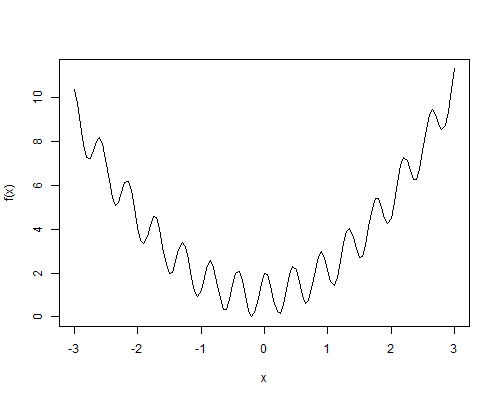
\includegraphics[width=\linewidth]{p7_1d.png}
\caption{Curva función objetivo}
\label{c4}
\end{subfigure}
\begin{subfigure}[b]{0.45\linewidth}
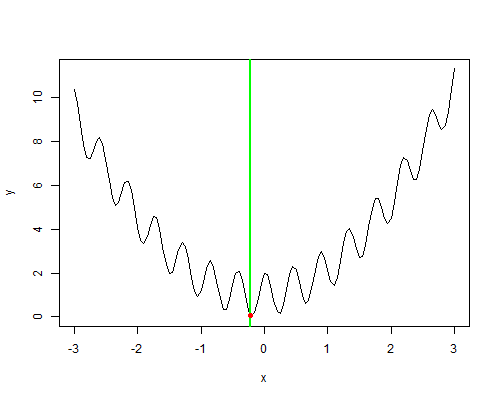
\includegraphics[width=\linewidth]{schaeffer.png}
\caption{Punto más bajo posible}
\label{c5}
\end{subfigure}
\caption{Función de la curva de Schaeffer donde se encuentra el punto tan abajo como posible}
    \label{Fig.1}
\end{figure}
En la figura \ref{c5} se muestra el punto más bajo posible, este código fue modificado con la finalidad de mostrar el punto más alto posible para realizar una comparación ver figura \ref{Fig.2} donde se maximiza el valor de la variable (figura \ref{2a}) y se modifica la función obteniendo menos simetría (figura \ref{2b}), el mayor valor que yo he visto se marcara con una línea y no se moverá si mi punto no ha tenido un valor mayor.
\begin{lstlisting}
g <- function(x, y) {
    return(((x + 0.5)^4 - 30 * x^2 - 20 * x + (y + 0.5)^4 - 30 * y^2 - 20 * y)/100)
repeticiones<-15
\end{lstlisting}
En el siguiente código se muestra la función de la curva que fue sustituida $n$ veces para comprender cual función tenia menos simetria.
\begin{figure}[h!]
    \centering
\begin{subfigure}[b]{0.45\linewidth}
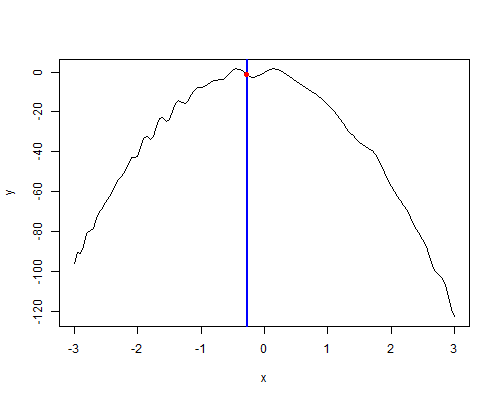
\includegraphics[width=\linewidth]{p7_t003.png}
\caption{Maximo punto de la variable}
\label{2a}
\end{subfigure}
\begin{subfigure}[b]{0.45\linewidth}
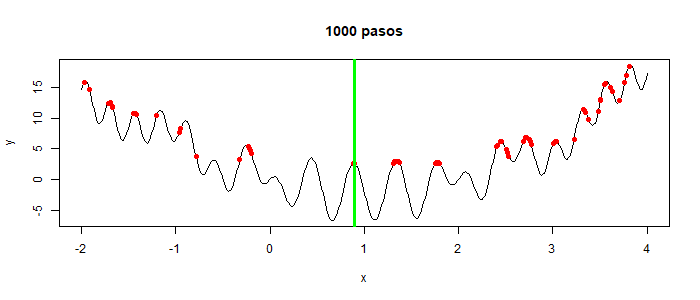
\includegraphics[width=\linewidth]{p7_1000.png}
\caption{Replicas de puntos más altos posibles modificando la función}
\label{2b}
\end{subfigure}
\caption{Función de la curva donde se encuentra el punto más alto como posible}
    \label{Fig.2}
\end{figure}

Para mayor visualización observar los archivos .gif en el repositorio de GitHub \cite{gitadrian}, ahora se requiere agregar una función tridimensional tal como se observa en la figura \ref{fig.3} y controlar el ángulo para observarlo desde la parte superior en dos direcciones marcando con un punto el mayor valor obtenido de por lo menos 15 replicas. En la figura \ref{fig.4} se muestran los resultados en mapas de calor de las 15 replicas en secuencias marcando con puntos de colores la posición máxima alcanzada, tal como se muestra en la figura \ref{4c} donde el valor maximo alcanzado sobre el eje z es muy cercano a $0$ para todas las replicas.
\begin{figure}[h!]
    \centering
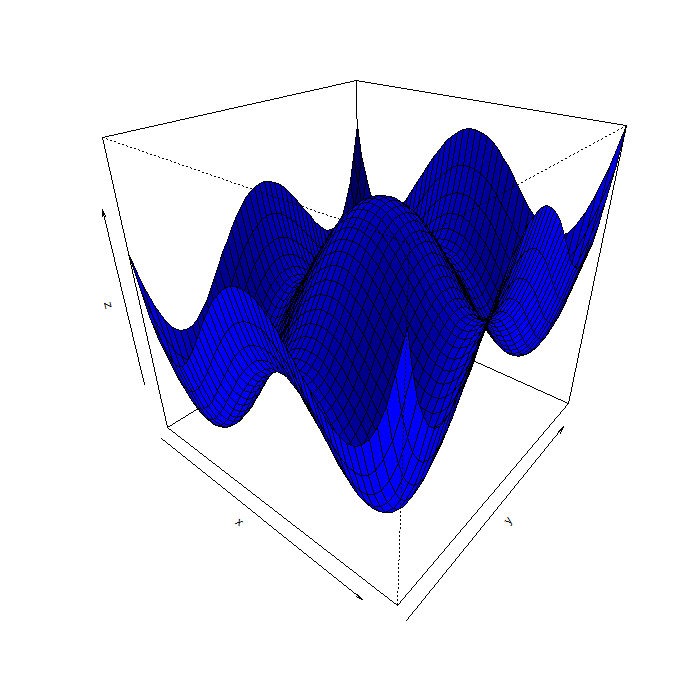
\includegraphics[width=70MM]{p7_2d.png}
\caption{Función tridimensional}
    \label{fig.3}
\end{figure}

\begin{figure}[h!]
    \centering
\begin{subfigure}[b]{0.45\linewidth}
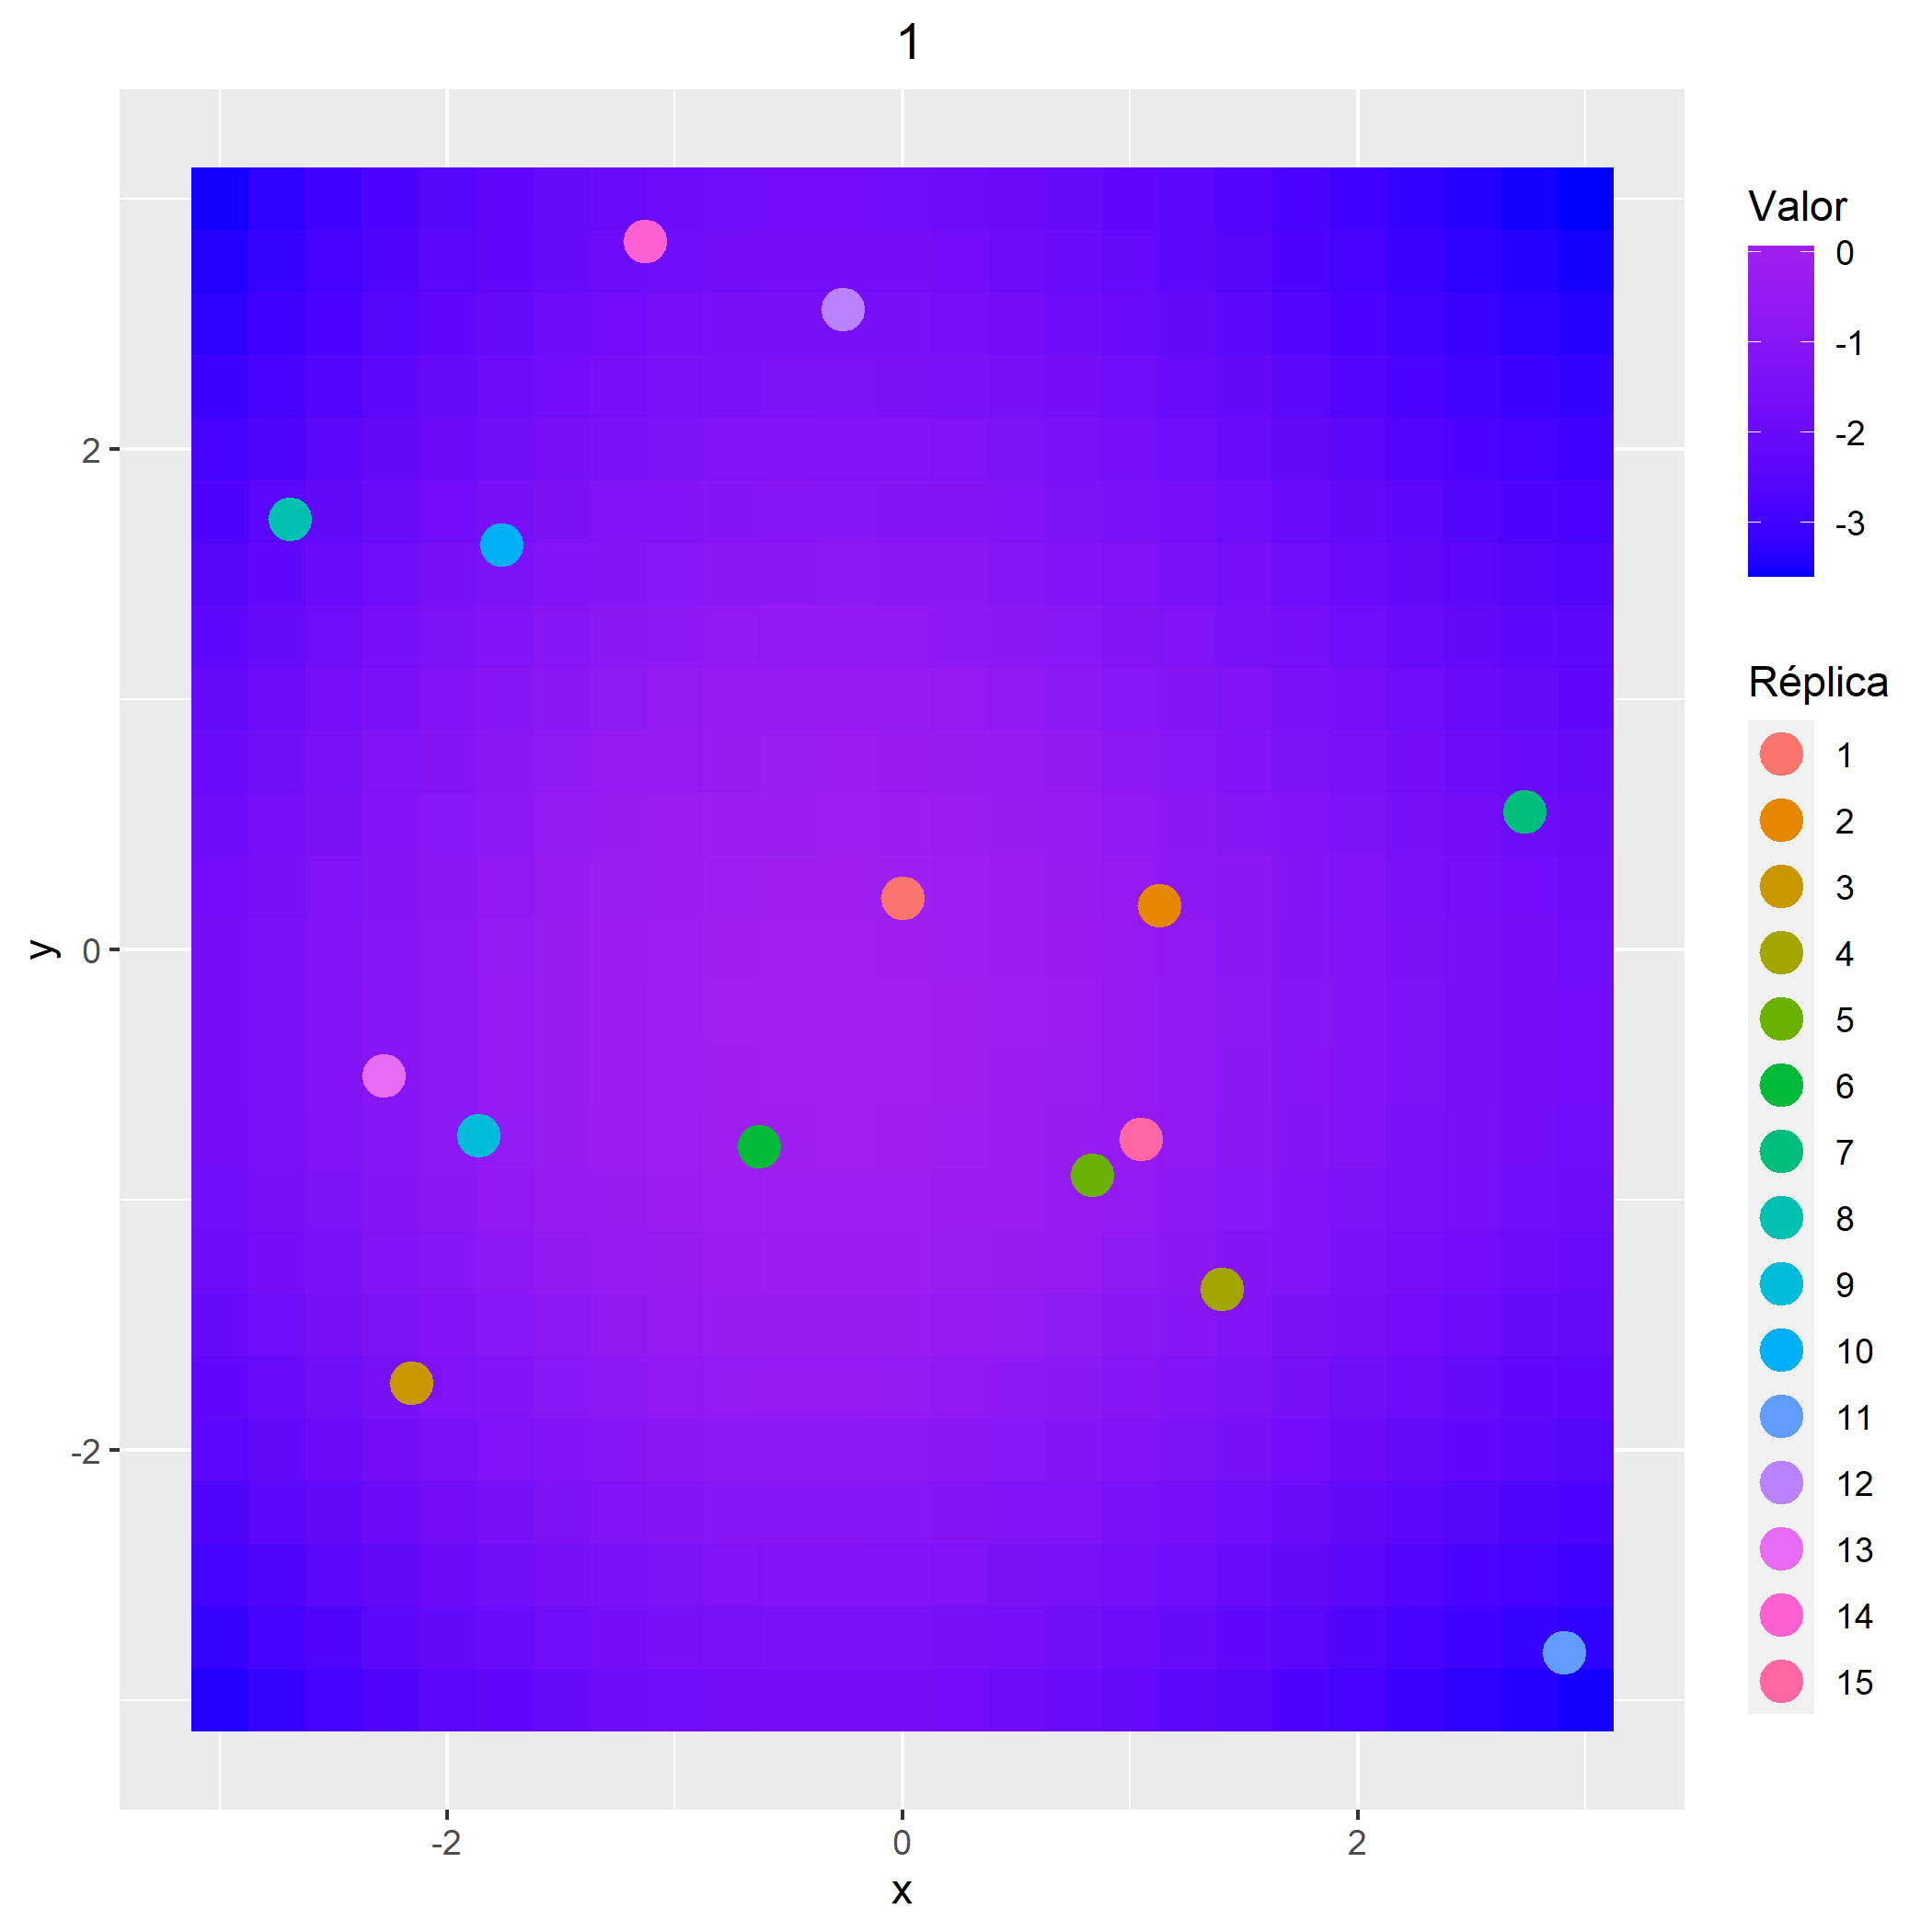
\includegraphics[width=\linewidth]{P7_paso_ 1 .png}
\caption{Máximo inicial sobre eje z}
\label{4a}
\end{subfigure}
\begin{subfigure}[b]{0.45\linewidth}
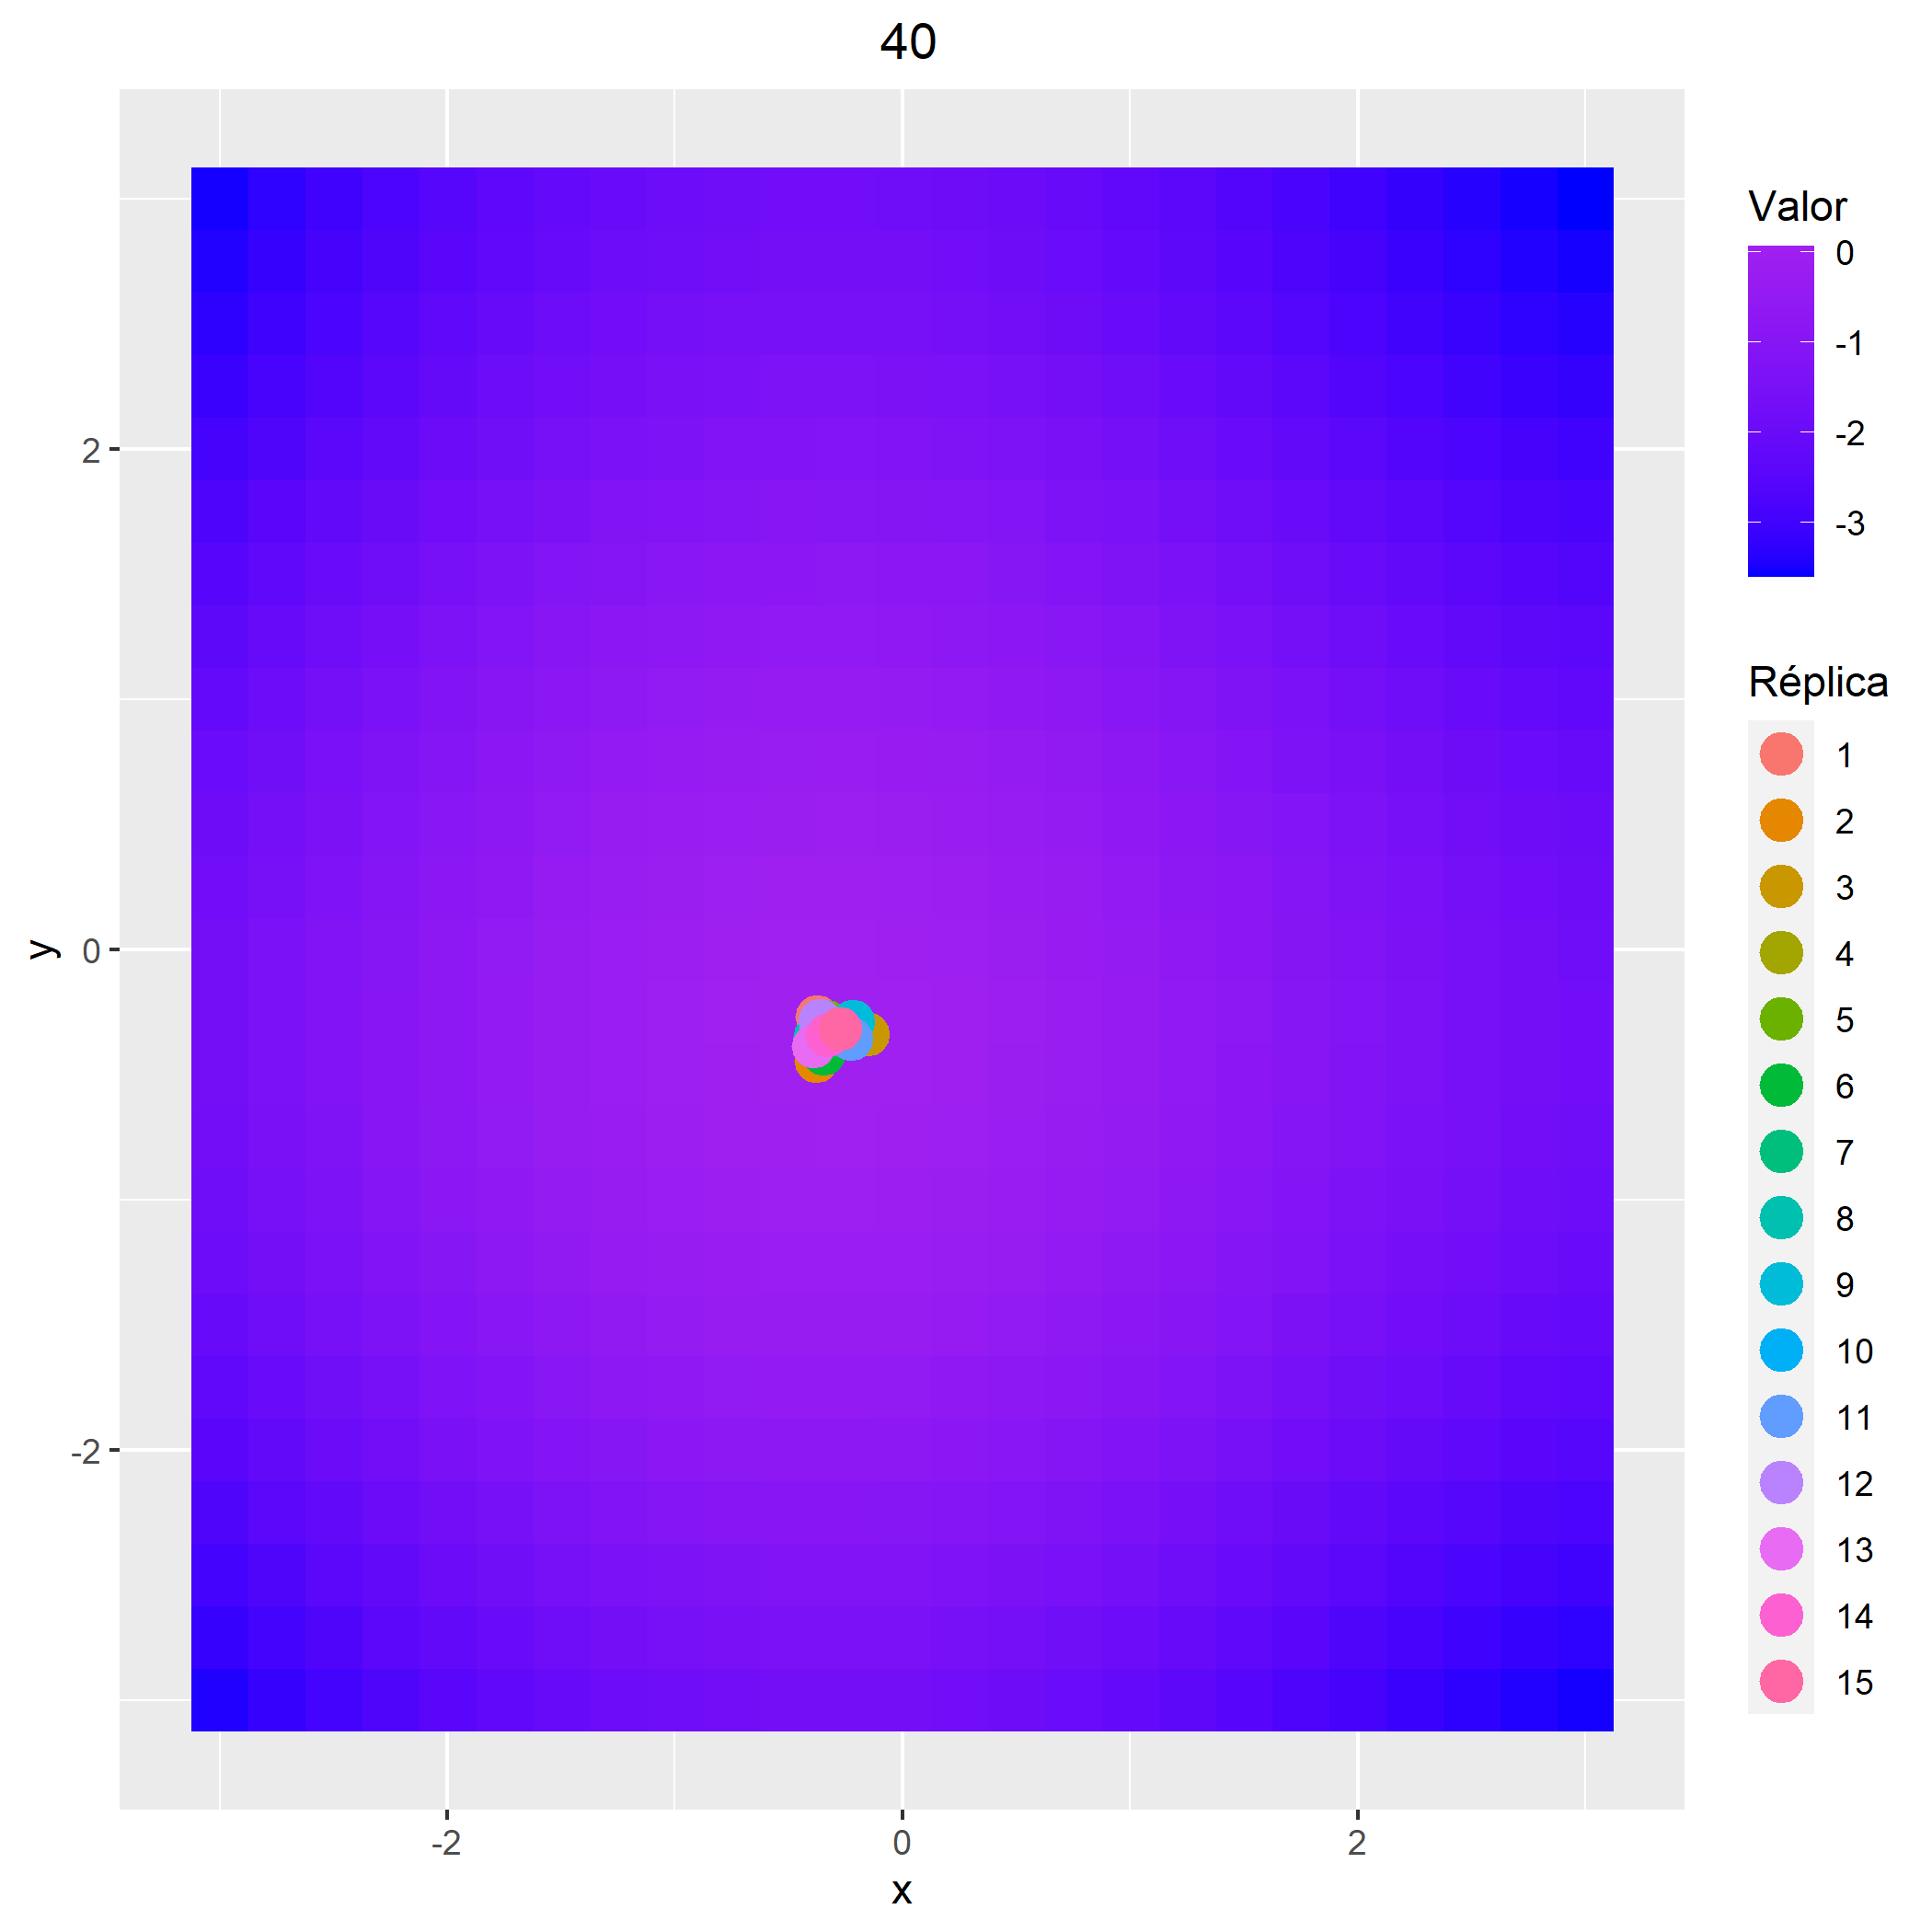
\includegraphics[width=\linewidth]{P7_paso_ 40 .png}
\caption{Máximo valor sobre eje z}
\label{4c}
\end{subfigure}
\caption{Mapa de calor de 15 replicas simultaneas con máximo valor en z}
    \label{fig.4}
\end{figure}



\section{Conclusión}
En cuanto tengamos un mayor numero de pasos de nuestro punto existe mayor probabilidad de alcanzar el punto más alto, dentro de los resultados de nuestro mapa de calor se muestra una cercancía al mayor valor de z que es $0$ tal como se muestra en la figura \ref{4c}.
\end{justify}
\newpage
\bibliography{p7} %\bibliography dentro de los corchetes aparece el comando seccion de referencias  sin embargo para que aparezca tiene que aparecer la seccion \bibliographystyle para dar un estilo del tipo de letra o tipo de acomodo que llevara 
\bibliographystyle{ieeetr}   %\da un estilo de acomodo dependiendo del comando dentro d corchetes
\end{document} %indica finalizacion de lo señalado en el parentesis en este caso el documento
